\documentclass{article}

\usepackage[margin=1in]{geometry}
\usepackage{amsmath,amsthm,amssymb}
\usepackage{bbm, enumerate, tikz}
\usepackage{multicol}

\newenvironment{problem}[2][Problem]{\begin{trivlist}
\item[\hskip \labelsep {\bfseries #1}\hskip \labelsep {\bfseries #2.}]}{\end{trivlist}}
\newenvironment{note}[1][Note.]{\begin{trivlist}
\item[\hskip \labelsep {\bfseries #1}]}{\end{trivlist}}

\begin{document}

\title{Fall 2013: Complex Analysis Graduate Exam}
\author{Peter Kagey}

\maketitle

% -----------------------------------------------------
% First problem
% -----------------------------------------------------
\begin{problem}{1}
  Compute \[
    \int_0^\infty \frac{\log^2 x}{1 + x^2}\,dx.
  \]
\end{problem}

\begin{proof}
  For ease of notation, name the integrand $f$; that is, \[
    f(z) = \frac{\log^2 z}{1 + z^2}.
  \]
  % Then $f$ has isolated singularities when $x^4 = e^{\pi i + 2\pi i k}$
  We will compute the integral by using the Residue Theorem together with (the
  limit of) a contour carefully designed to avoid the singularity at the
  origin, and including one of the simple poles of $f$:
  \begin{multicols}{2}
  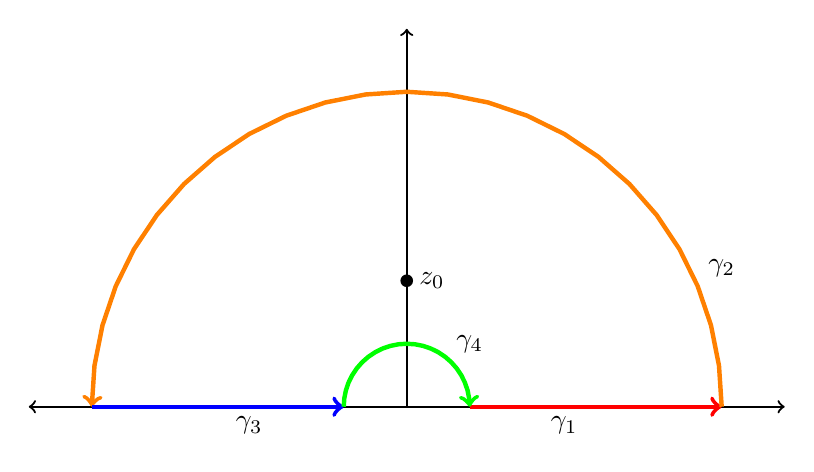
\begin{tikzpicture}[scale=0.8]
    % \draw[very thin,color=gray] (-0.9,-0.9) grid (5.9,5.9);
    \draw[thick, <->] (-6,0)--(6,0);
    \draw[thick, ->] (0,0)--(0,6);
    \fill (0,2) circle (0.1);
    \draw node at (0.4, 2) {$z_0$};
    \draw[ultra thick, ->, draw=red, domain=1:5] plot ({\x}, {0});
    \draw node at (2.5, -0.3) {$\gamma_{1}$};
    \draw[ultra thick, ->, draw=orange, domain=0:180] plot ({5*cos(\x)}, {5*sin(\x)});
    \draw node at (5, 2.2) {$\gamma_{2}$};
    \draw[ultra thick, <-, draw=blue, domain=1:5] plot ({-\x}, 0);
    \draw node at (-2.5, -0.3) {$\gamma_{3}$};
    \draw[ultra thick, ->, draw=green, domain=180:0] plot ({cos(\x)}, {sin(\x)});
    \draw node at (1, 1) {$\gamma_{4}$};
  \end{tikzpicture}\\
  \begin{align}
    \gamma_{1} &= \{t + 0i\ |\ x \in [\varepsilon, R] \} \\
    \gamma_{2} &= \{R e^{it}\ |\ t \in [0,\pi] \} \\
    \gamma_{3} &= \{0 + ti\ |\ t \in [-R, -\varepsilon]\} \\
    \gamma_{4} &= \{\varepsilon e^{-it}\ |\ t \in [-\pi, 0]\}.
  \end{align}
  \end{multicols}
  For small $\epsilon$ and large $R$, this contour encloses a
  single simple pole of $f$, namely $z_0 = i$.
  \[
    \int_{\gamma_1} f(z)\,dz +
    \int_{\gamma_2} f(z)\,dz +
    \int_{\gamma_3} f(z)\,dz +
    \int_{\gamma_4} f(z)\,dz =
    2\pi i \operatorname{Res}_i(f).
  \]
\end{proof}
In the limit, the integrals over each arcs ($\gamma_2$ and $\gamma_4$) vanishes.
\begin{align*}
  \left|\int_{\gamma_2}f(z)\,dz\right|
  &= \left|
    \int_0^{\pi}\frac{\log^2(Re^{it})}{1 + R^2e^{2it}}iRe^{it}\,dt
  \right|\\
  &\leq \int_0^{\pi}\left|
    \frac{\log^2(Re^{it})}{1 + R^2e^{2it}}iRe^{it}
  \right|\,dt \\
  &\leq \int_0^{\pi}\left|
    \frac{\log^2(Re^{it})}{R}
  \right|\,dt \\
  &\leq \int_0^{\pi}\left|
    \frac{\log^2(R) + 2it\log(R) - t}{R}
  \right|\,dt
\end{align*} which vanishes by the $ML$ inequality as $R \rightarrow \infty$.
Similarly, \begin{align*}
  \left|\int_{\gamma_2}f(z)\,dz\right|
  &= \left|
    \int_0^{\pi}\frac{\log^2(\varepsilon e^{it})}{1 + \varepsilon ^2e^{2it}}i\varepsilon e^{it}\,dt
  \right|\\
  &\leq \int_0^{\pi}\left|
    \frac{\log^2(\varepsilon e^{it})}{1 + \varepsilon ^2e^{2it}}i\varepsilon e^{it}
  \right|\,dt \\
  &\leq \int_0^{\pi}\left|
    \frac{\log^2(\varepsilon e^{it})}{1}i\varepsilon e^{it}
  \right|\,dt \\
  &\leq \int_0^{\pi}\left|
    \varepsilon\log^2(\varepsilon e^{it})
  \right|\,dt \\
  &\leq \int_0^{\pi}\left|
    \varepsilon(\log^2(\varepsilon) + 2it\log(\varepsilon) + t)
  \right|\,dt,
\end{align*} which also vanishes as $\varepsilon \rightarrow 0$ by the ML
inequality, as can be seen by two applications of L'H\^opital's rule:
\begin{align*}
  \lim_{\varepsilon \rightarrow 0} \varepsilon\log^2(\varepsilon)
  &= \lim_{\varepsilon \rightarrow 0} \frac{\log^2(\varepsilon)}{\varepsilon^{-1}} \\
  &= \lim_{\varepsilon \rightarrow 0} \frac{2\log(\varepsilon)\varepsilon^{-1}}{-\varepsilon^{-2}}\\
  &= \lim_{\varepsilon \rightarrow 0} \frac{2\log(\varepsilon)}{-\varepsilon^{-1}} \\
  &= \lim_{\varepsilon \rightarrow 0} \frac{2\varepsilon^{-1}}{\varepsilon^{-2}} \\
  &= \lim_{\varepsilon \rightarrow 0} 2\varepsilon \\
  &= 0.
\end{align*}
This means that our equation simplifies in the limit to \[
  \int_{\gamma_1} f(z)\,dz +
  \int_{\gamma_3} f(z)\,dz =
  2\pi i \operatorname{Res}_i(f).
\] And the left-hand side further simplifies to \begin{align*}
  \int_\varepsilon^R\frac{\log^2 z}{1 + z^2}\,dz
  + (-1)\int_R^\varepsilon\frac{\log^2(-z)}{1 + (-z)^2}\,dz &=
  \int_\varepsilon^R\frac{\log^2 z + \log^2(-z)}{1 + z^2}\,dz \\
  &= \int_\varepsilon^R\frac{\log^2 z + (\log(z) + \log(-1))^2}{1 + z^2}\,dz \\
  &= 2\int_{\gamma_1} f(z)\,dz + \int_\varepsilon^R\frac{2\pi i\log(z)}{1 + z^2}\,dz + \int_\varepsilon^R\frac{-\pi^2}{1 + z^2}\,dz
\end{align*}
So by the Residue Theorem, the integral evaluates to \[
  \int_0^\infty\frac{\log^2 z}{1 + z^2}\,dz
  = \pi i \operatorname{Res}_i(f)
    - \underbrace{\pi i\int_0^\infty\frac{\log(z)}{1 + z^2}\,dz}_\text{purely imaginary}
    - \frac{1}{2}\int_0^\infty\frac{-\pi^2}{1 + z^2}\,dz,
\] and by only considering the real part, it is enough to compute the residue and the last integral: \[
  \operatorname{Res}_i(f)
  = \frac{\log^2(i)}{2i}
  = \frac{(\pi i/2)^2}{2i}
  = \frac{i\pi^2}{8},
\] and \[
  -\pi^2\int_\varepsilon^R\frac{1}{1 + z^2}\,dz = -\frac{\pi^3}{2}
\]
Therefore \begin{align*}
  \int_0^\infty\frac{\log^2 z}{1 + z^2}\,dz
  &= \pi i \left(\frac{i\pi^2}{8}\right)
    - \frac{1}{2}\left(-\frac{\pi^3}{2}\right) \\
  &= -\frac{\pi^3}{8} + \frac{\pi^3}{4} \\
  &= \frac{\pi^3}{8}.
\end{align*}
% -----------------------------------------------------
% Second problem
% -----------------------------------------------------
\pagebreak

\begin{problem}{2}
  Find the number of \textit{distinct} zeros of $f(z) = z^6 + (10 - i)z^4 + 1$
  inside $(-1, 1)\times(-1,1)$.
\end{problem}

\begin{proof}
  First, we will use Rouch\'e's Theorem to establish a bound on the number of
  roots (with multiplicity) inside of the region $D = (-1, 1)\times(-1,1)$.

  For a lower bound, we will count the number of roots inside $|z| = 1$ and
  for an upper bound, we will count the number of roots inside $|z| = \sqrt2$.
  In both cases we will compare against the function $g(z) = (10 - i)z^4 + 1$.

  \textbf{(Case 1: $|z| = 1$)} Notice that when $|z| = 1$, \begin{align*}
    |f - g| = |z^6| &= 1\\
    &< |(10 - i)z^4| - |z^6| - 1 = |10 - i| - 2 \\
    &< |f|,
  \end{align*} by the triangle inequality.
  So $f$ and $g$ have the same number of roots inside the unit disk, and $g$
  has all four roots inside the unit disk: \begin{align*}
    g(z) &= (10 - i)z^4 + 1 = 0 \\
    |z| &= \left|\frac{-1}{10 - i}\right|^{1/4} < 1.
  \end{align*}
  Thus $f$ has at least four roots in $D$.

  \textbf{(Case 2: $|z| = \sqrt2$)} When $|z| = \sqrt2$, \begin{align*}
  |f - g| = |z^6| &= 8\\
  &< |(10 - i)z^4| - |z^6| - 1 = 4|10 - i| - 8 - 1 \\
  &< |f|,
  \end{align*} by the triangle inequality.
  And since $g$ has all four roots inside the unit disk, it certainly has
  all roots inside the disk of radius $\sqrt2$.
  \\
  Now that we have established that $f$ has four roots inside $D$, it remains
  to check multiplicity, which can be done by comparing the roots of $f$
  and $f'$ inside of $D$.
  \\
  Notice that $f'(z) = 6z^5 + 4(10 - i)z^3$ factors as
  $f'(z) = z^3(6z^2 + 40 - 4i)$. Clearly $f$ does not have any roots at $z = 0$,
  so it is enough to check the roots of $6z^2 + 40 - 4i$. \begin{align*}
  z^2 = \frac{40 - 4i}{6} \\
  |z| = \left|\frac{40 - 4i}{6}\right|^{1/2} > \sqrt6.
  \end{align*}
  Therefore $f'(z)$ does not share any roots with $f(z)$ inside $D$, and so
  all roots inside $D$ are distinct. Thus $f$ has exactly four distinct roots
  inside $D$.
\end{proof}

% -----------------------------------------------------
% Third problem
% -----------------------------------------------------
\pagebreak

\begin{problem}{3}
  Supposer that $f$ is holomorphic in a neighborhood $U$ of $a \in \mathbb C$.
  Conside the following two statements.
  \begin{enumerate}[(i)]
    \item There exist two sequences $\{z_k\}_{k=1}^\infty$ and
    $\{w_k\}_{k=1}^\infty$ in $U \setminus \{a\}$ converging to $a$ such that
    $z_k \neq w_k$ and $f(z_k) = f(w_k)$ for all $k \in \mathbb N$.
    \item $f'(a) = 0$.
  \end{enumerate}
\end{problem}

\begin{proof}
\end{proof}

% -----------------------------------------------------
% Fourth problem
% -----------------------------------------------------
\pagebreak

\begin{problem}{4}
  Let $f$ be analytic in an open set $U \subseteq \mathbb C$, and let
  $K \subseteq U$ be compact. Shw that there exists a constant $C$ depending on
  $U$ and $K$ such that \[
    |f(z)| \leq C\left(\int_U|f|^2\right)^{1/2}
  \] for all $z \in K$.
\end{problem}

\begin{proof}
\end{proof}

\end{document}
